\section{Νέος μικροελεγκτής}
\label{sec:example3}

Όπως και στο προηγούμενο παράδειγμα, έτσι και σε αυτό, σε περίπτωση που ο χρήστης θέλει να χρησιμοποιήσει κάποιον μικροελεγκτή για τον οποίο δεν υπάρχει υλοποίηση στην παρούσα εργασία, θα πρέπει να κάνει κάποια έξτρα βήματα.

Αυτή η περίπτωση επέκτασης, είναι λιγότερο χρονοβόρα από την προηγούμενη, καθώς το μόνο που χρειάζεται να γίνει από πλευράς του χρήστη, είναι να δημιουργήσει το αρχείο που γράφεται στην γλώσσα στην οποία αναπτύχθηκε στα πλαίσια της εργασίας, και περιγράφει την εκάστοτε συσκευή. Από κει και πέρα, εφόσον θέλει να χρησιμοποιήσει περιφερειακά που ήδη υποστηρίζονται, δε χρειάζεται τίποτα επιπλέον, καθώς ο κώδικας σε C που είναι απαραίτητος ώστε να λειτουργήσουν, είναι ήδη υλοποιημένος.

Έστω λοιπόν ότι ο χρήστης θέλει να χρησιμοποιήσει τον μικροελεγκτή WeMos D1 mini Pro ESP8266. Αν στο αρχείο (.con) όπου δηλώνονται οι συνδέσεις του κάθε περιφερειακού με τον μικροελεγκτή, συμπεριλάβει τον ελεγκτή αυτόν, τότε η εντολή για την παραγωγή κώδικα θα επιστρέψει το μήνυμα που φαίνεται στο \autoref{fig:error_message3}, καθώς δεν υπάρχει έτοιμη υλοποίηση.

\begin{figure}[!ht]
	\centering
	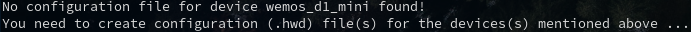
\includegraphics[width=0.8\textwidth]{./images/chapter6/error_message3.png}
	\caption{Μήνυμα για συσκευή που δεν υποστηρίζεται}
	\label{fig:error_message3}
\end{figure}

Άρα λοιπόν και πάλι ο χρήστης πρέπει να δημιουργήσει ένα .hwd αρχείο, όπου θα περιγράφει τα χαρακτηριστικά του μικροελεγκτή (σύμφωνα με τη γλώσσα που υλοποιήθηκε στην παρούσα εργασία).

Το περιεχόμενο του αρχείου θα μπορούσε να είναι το ακόλουθο.

\begin{lstlisting}
board:
	name: wemos_d1_mini
	vcc: 3.3
	operating_voltage: 3.3
	memory:
	flash: 16 mb
	cpu:
	cpu_family: ESP8266
	max_freq: 160 mhz
	fpu: false
	network:
	- wifi:
		name: wifi_1
		freq: 2.5 ghz
	pins:
	- io_pin: ->
		name: rst
		number: 1
	- io_pin: -> adc
		name: a0
		number: 2
		vmax: 3.2
	- io_pin: -> gpio
		name: d0
		number: 3
	- io_pin: -> gpio, sck-0
		name: d5
		number: 4
	- io_pin: -> gpio, miso-0
		name: d6
		number: 5
	- io_pin: -> gpio, mosi-0
		name: d7
		number: 6
	- io_pin: -> gpio, cs-0
		name: d8
		number: 7
	- power:
		name: power_3v3
		number: 8
		type: 3v3
	- io_pin: -> tx-0
		name: tx
		number: 9
	- io_pin: -> rx-0
		name: rx
		number: 10
	- io_pin: -> gpio, scl-0
		name: d1
		number: 11
	- io_pin: -> gpio, sda-0
		name: d2
		number: 12
	- io_pin: -> gpio
		name: d3
		number: 13
	- io_pin: -> gpio
		name: d4
		number: 14
	- power:
		name: gnd
		number: 15
		type: gnd
	- power:
		name: power_5v
		number: 16
		type: 5v
\end{lstlisting}

Αφού συμπληρωθεί αυτό το αρχείο, τότε πλέον ο μικροελεγκτής αυτός υποστηρίζεται πλήρως, και άρα μπορεί να χρησιμοποιηθεί σαν όρισμα στη διαδικασία.